%http://www.tablesgenerator.com/latex_tables

Para el análisis de las rutas nos centraremos principalmente en el RTT y ZRTT de cada Gateway atravesado. Es importante mencionar que no todos los Gateways emiten una respuesta a los paquetes ICMP emitidos ya que algunos podrían no tener implementada esa funcionalidad. Por esta razón se verá más adelante que los TTL presentados en las tablas no crecen de a uno.

Para calcular el RTT de cada Gateway envíamos numerosos paquetes al mismo para obtener un promedio. Determinamos que envíar 20 paquetes por cada salto era suficiente. También se calculó el desvío estandar:
\newline
\newline
$RTT=\frac{\sum_{i=1}^{20}{RTT_i}}{20}$
\newline
$\sigma = \frac{\sum_{i=1}^{20}{(RTT_i-RTT)^2}}{20}$
\newline

Además del RTT se obtuvo el ZRTT para cada Gateway. Este valor nos permite analizar si un determinado Gateway tiene un RTT mayor o menor a la media con respecto a la ruta global, dependiendo de si el ZRTT es positivo o negativo. Por lo tanto es una muy buena herramienta para analizar si se trata de un enlace submarino. Fue calculado de la siguiente manera:
\newline
\newline
$ZRTT_i = \frac{RTT_i-\overline{RTT}}{SRTT}$
en donde $RTT_i$ es el $RTT$ promedio calculado para cada salto, $\overline{RTT}$ es el $RTT$ promedio de la ruta global y $SRTT$ es el desvío estándar de la ruta global.
\newline

Para verificar si los valores de RTT y ZRTT se corresponden con la realidad decidimos utilizar una herramienta de geolocalización de modo que podamos determinar la ubicación aproximada de un Gateway. De esta forma nos era posible verificar, por ejemplo, si a valores grandes de ZRTT para determinado Gateway le correspondia una ubicación alejada de nuestro origen. También incluimos, para cada ruta analizada, un mapa en donde pueden verse los lugares por donde van pasando los paquetes.

A continuación, los resultados obtenidos:

\subsection{Universidad de Australia}

\begin{table}[H]
\begin{tabular}{llllll}
TTL & IP              & RTT(prom)        & Desviacion Estandar & ZRTT            & Location                \\
1   & 192.168.1.1     & 1.58843994141 ms & 0.223531225414      & -1.71303307932  & *                       \\
2   & 190.245.25.1    & 42.6805853844 ms & 19.8176943898       & -1.40040003076  & Argentina               \\
6   & 200.89.165.49   & 29.913687706 ms  & 11.1214135157       & -1.49753183293  & Argentina               \\
7   & 200.89.165.250  & 31.9589853287 ms & 13.8956215103       & -1.48197100922  & Argentina               \\
8   & 64.209.94.97    & 25.0925540924 ms & 14.3493883219       & -1.53421148747  & United States           \\
9   & 67.16.139.18    & 160.412049294 ms & 25.8748003019       & -0.504687575834 & United States           \\
10  & 64.208.27.102   & 186.840640174 ms & 10.0093951121       & -0.303616279922 & United States           \\
11  & 129.250.3.172   & 188.704538345 ms & 16.1066140831       & -0.289435560925 & United States:Englewood \\
12  & 129.250.3.174   & 194.419503212 ms & 17.2554007517       & -0.245955551074 & United States:Englewood \\
13  & 129.250.2.168   & 194.349682331 ms & 17.6758535646       & -0.246486755143 & United States:Englewood \\
14  & 129.250.2.230   & 198.079133034 ms & 15.9807483604       & -0.218112730617 & United States:Englewood \\
15  & 204.1.253.166   & 193.757641315 ms & 13.2299664539       & -0.250991060907 & United States:Englewood \\
16  & 202.158.194.172 & 319.028556347 ms & 14.9289581536       & 0.702082273172  & Australia               \\
17  & 113.197.15.68   & 318.016040325 ms & 13.9356377591       & 0.694378952569  & Australia               \\
18  & 113.197.15.66   & 349.911153316 ms & 12.0683422641       & 0.937040081626  & Australia               \\
19  & 113.197.15.65   & 352.194654942 ms & 14.7653444091       & 0.954413184605  & Australia               \\
20  & 202.158.193.146 & 353.731060028 ms & 10.920976595        & 0.966102304286  & Australia               \\
21  & 202.158.193.186 & 358.153343201 ms & 18.3398195658       & 0.999747465787  & Australia               \\
22  & 137.111.189.4   & 361.728382111 ms & 13.9907095978       & 1.02694671034   & Australia               \\
23  & 137.111.13.200  & 357.019650936 ms & 13.0007013927       & 0.991122224516  & Australia:Ryde          \\
24  & 137.111.223.12  & 387.044274807 ms & 65.604054602        & 1.21955248999   & Australia               \\
25  & 137.111.223.158 & 383.823335171 ms & 60.9346988401       & 1.19504726723   & Australia              
\end{tabular}
\caption{Ruta hacia la universidad de Australia}
\label{my-label}
\end{table}

Notar que a medida que los TTL's se van incrementando también lo hacen el RTT y ZRTT. Esto era esperado que sucediera ya que los Gateways se encuentran cada vez más lejos del origen. Este comportamiento podrá verse mejor en los siguientes gráficos.

\begin{figure}[H]
	\begin{center}
		  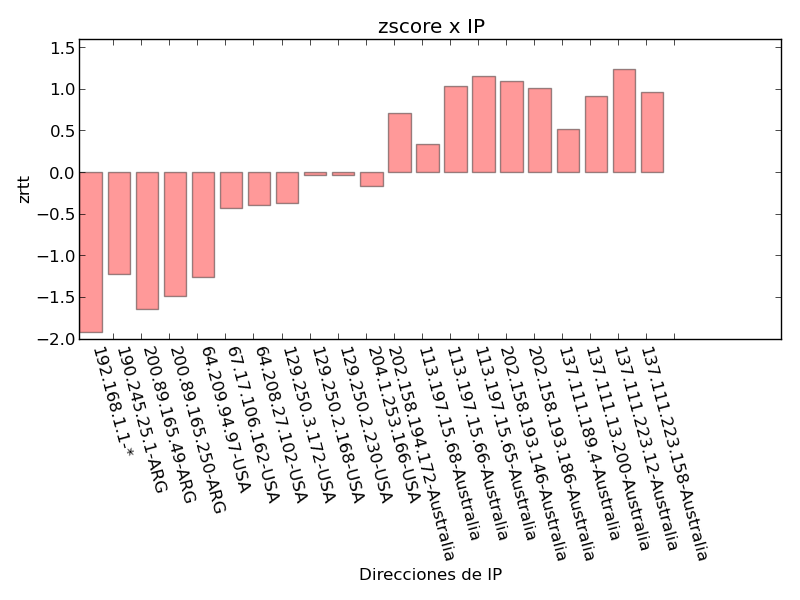
\includegraphics[scale=0.5]{../graficos_informe/mq_zscore.png}
		  \caption{ZRTT para cada Gateway}
		  \label{fig:contra1}
	\end{center}
\end{figure}

Aquí puede observarse claramente que a partir del Gateway que se encuentra localizado en Australia, el ZRTT se torna positivo. Esto indica, como mencionamos anteriormente, que el RTT para estos Gateways es mayor a la media de la ruta global lo cual tiene sentido ya que atraviesan un enlace submarino.

\begin{figure}[H]
	\begin{center}
		  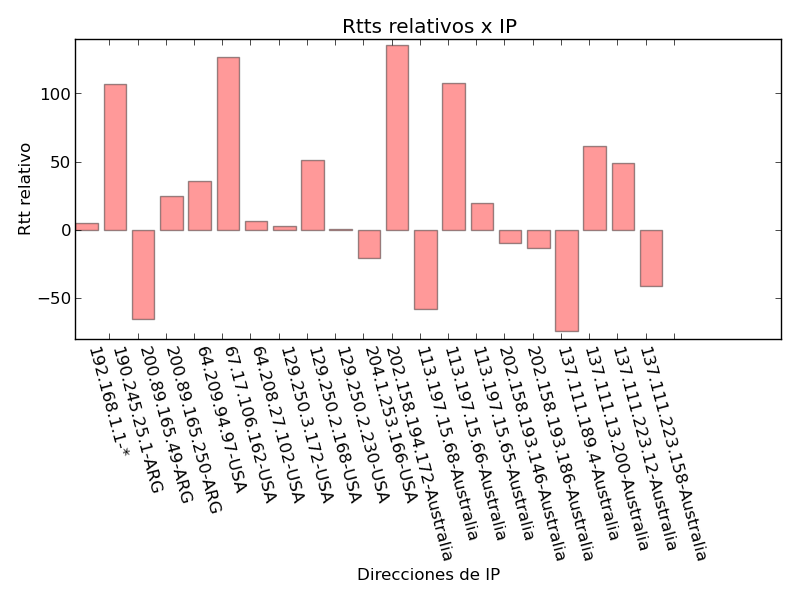
\includegraphics[scale=0.5]{../graficos_informe/mq_rtt.png}
		  \caption{RTT promedio para cada Gateway con el respectivo desvío estándar}
		  \label{fig:contra1}
	\end{center}
\end{figure}

Podemos ver en este gráfico que los RTT's van creciendo a medida que vamos hacia la derecha del gráfico.

\begin{figure}[H]
	\begin{center}
		  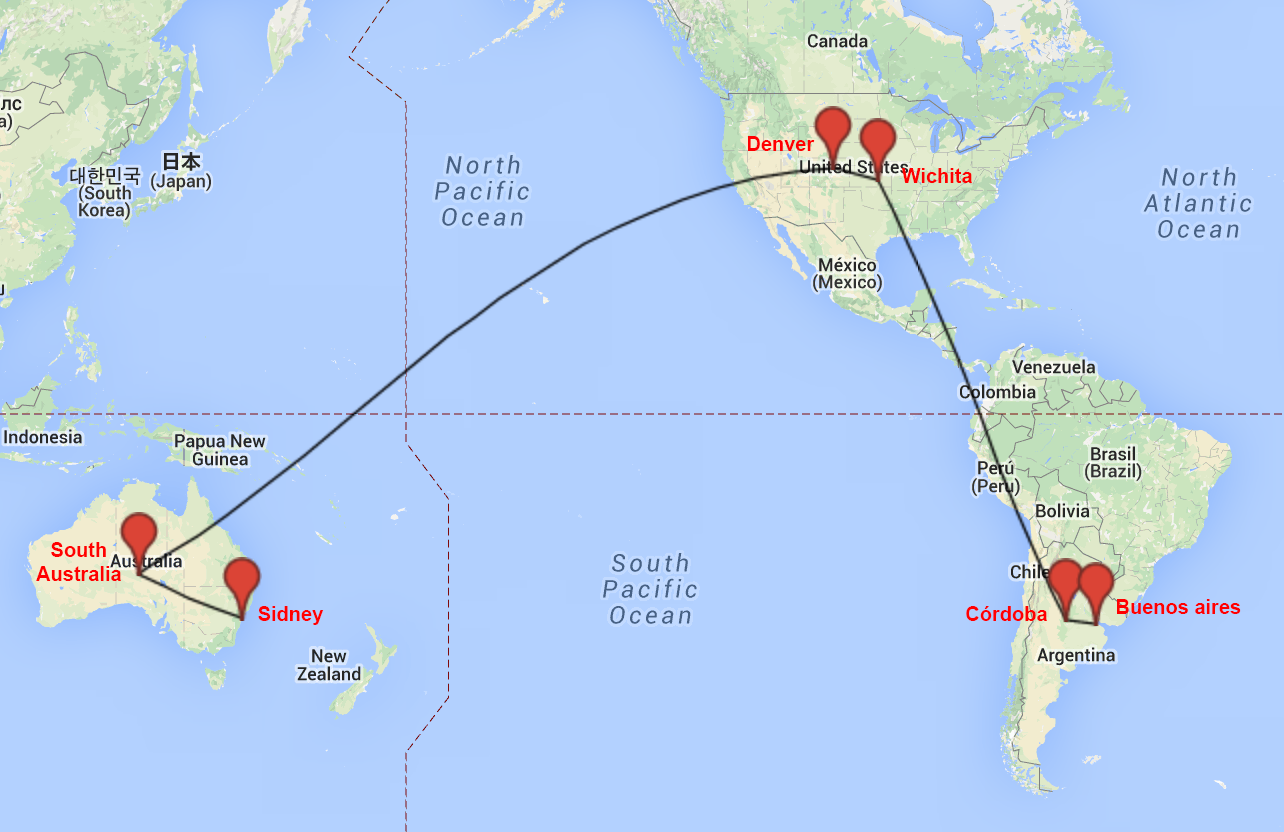
\includegraphics[scale=0.4]{../mapas/mapa_md.png}
		  \caption{Mapa de la ruta atravesada para llegar a la universidad de Australia}
		  \label{fig:contra1}
	\end{center}
\end{figure}

\subsection{Universidad de Kamchatka}

\begin{table}[H]
\begin{tabular}{llllll}
TTL & IP             & RTT(prom)        & Desviacion Estandar & ZRTT             & Location                     \\
1   & 192.168.1.1    & 1.80819829305 ms & 0.731853407234      & -1.08128839049   & *                            \\
2   & 190.245.25.1   & 17.3818061226 ms & 7.90250397557       & -1.04406066319   & Argentina                    \\
6   & 200.89.165.13  & 15.9910202026 ms & 6.77291322606       & -1.04738524921   & Argentina                    \\
7   & 200.89.165.2   & 14.0871167183 ms & 4.38023412359       & -1.05193641042   & Argentina                    \\
8   & 200.89.165.86  & 17.4869894981 ms & 4.67752646672       & -1.04380922896   & Argentina                    \\
9   & 195.22.220.174 & 18.2276844978 ms & 7.78620781179       & -1.04203864428   & Italy                        \\
10  & 89.221.34.255  & 272.055315971 ms & 12.2568505401       & -0.435279699866  & Italy                        \\
11  & 195.22.214.27  & 281.684625149 ms & 13.1891077384       & -0.412261443588  & Italy                        \\
12  & 95.167.92.6    & 413.393509388 ms & 6.4724957906        & -0.0974196625449 & Russian Federation           \\
13  & 87.226.223.206 & 419.344055653 ms & 7.38855122796       & -0.0831952569936 & Russian Federation           \\
14  & 85.28.192.185  & 957.480251789 ms & 4.33259948094       & 1.20318538023    & Russian Federation           \\
15  & 85.28.192.94   & 995.981001854 ms & 102.629633848       & 1.29521899506    & Russian Federation           \\
16  & 85.28.192.173  & 979.524040222 ms & 17.6097548431       & 1.2558796662     & Russian Federation           \\
17  & 85.28.192.90   & 950.519025326 ms & 6.6846143214        & 1.1865450074     & Russian Federation           \\
18  & 77.82.16.83    & 947.636032104 ms & 7.30217338762       & 1.17965339393    & Russian Federation:Kamchatka \\
19  & 85.28.217.202  & 963.758111 ms    & 8.51265755857       & 1.21819220673    & Russian Federation          
\end{tabular}
\caption{Ruta hacia la universidad de Kamchatka}
\label{my-label}
\end{table}

\begin{figure}[H]
	\begin{center}
		  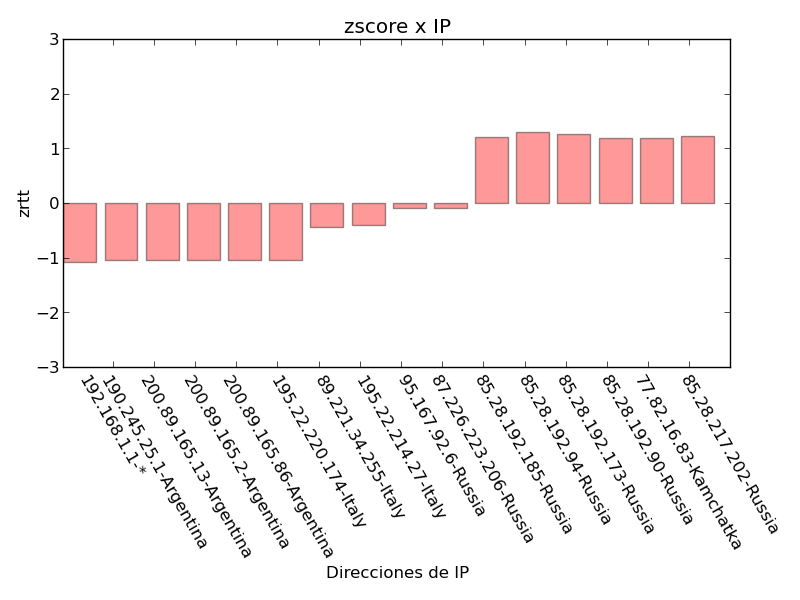
\includegraphics[scale=0.5]{../graficos_informe/kamgu_zscore.png}
		  \caption{ZRTT para cada Gateway}
		  \label{fig:contra1}
	\end{center}
\end{figure}

En este caso notamos que el ZRTT se torna positivo recién cuando el paquete atraviesa Rusia y no Italia. Sin embargo, notamos un aumento progresivo del ZScore.

\begin{figure}[H]
	\begin{center}
		  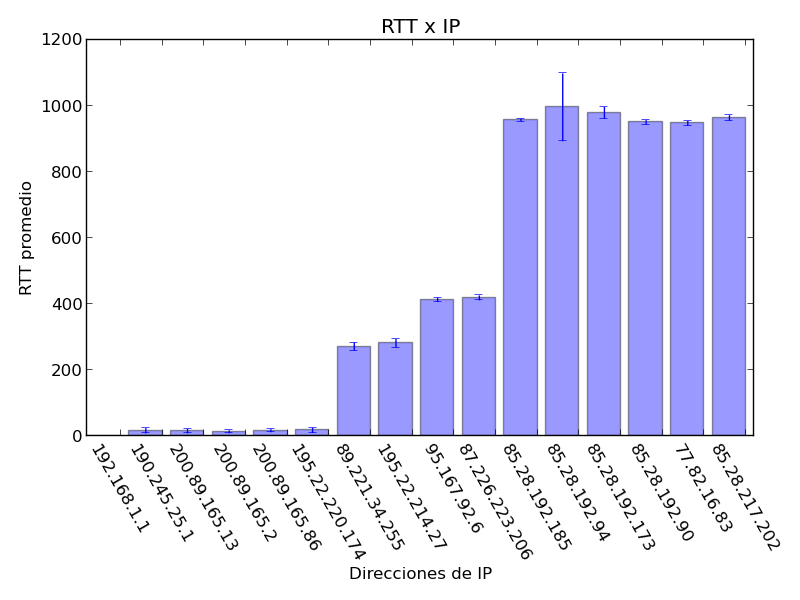
\includegraphics[scale=0.5]{../graficos_informe/kamgu_rtt.png}
		  \caption{RTT promedio para cada Gateway con el respectivo desvío estándar}
		  \label{fig:contra1}
	\end{center}
\end{figure}

Al igual que antes, puede observarse un crecimiento hacia la derecha. Notar la gran diferencia que hay entre los RTT's de un Gateway argentino y uno ruso.

\begin{figure}[H]
	\begin{center}
		  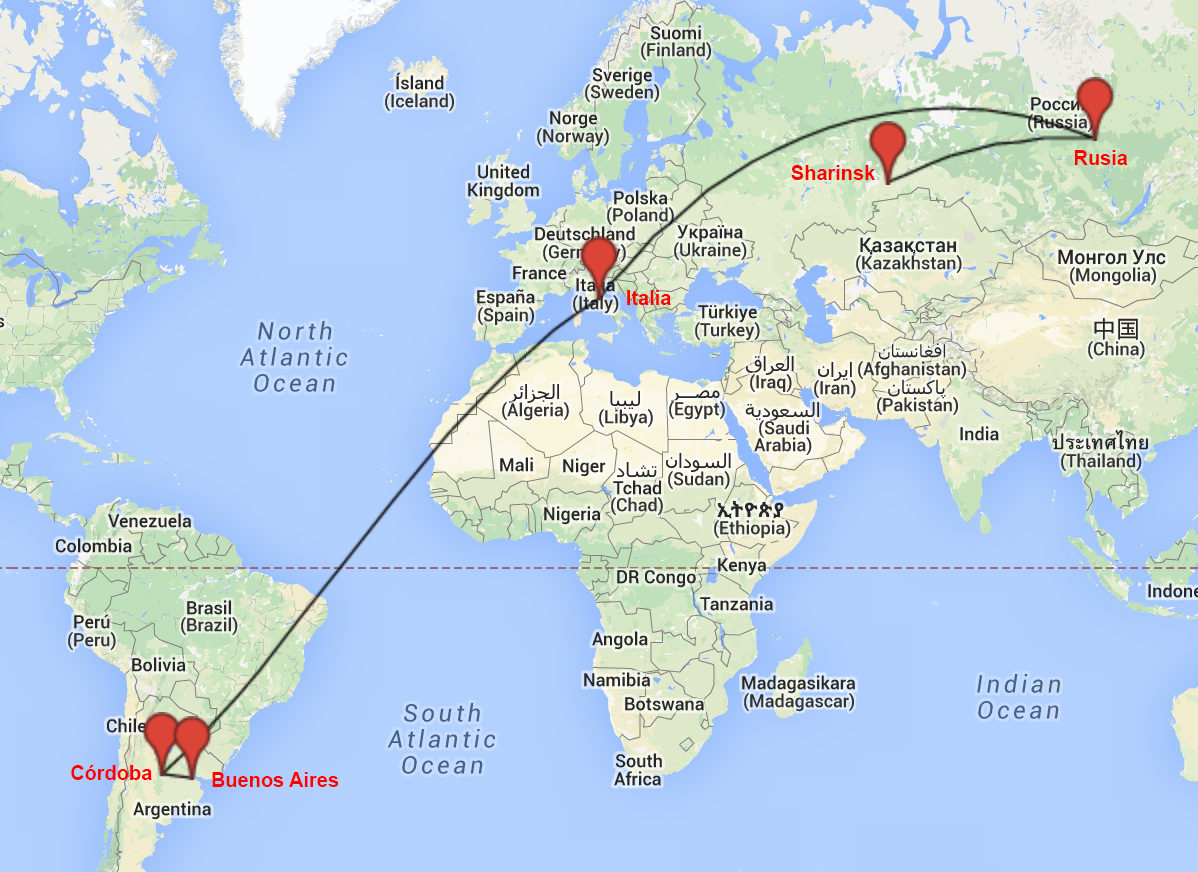
\includegraphics[scale=0.4]{../mapas/mapa_kamgu.png}
		  \caption{Mapa de la ruta atravesada para llegar a la universidad de Kamchatka}
		  \label{fig:contra1}
	\end{center}
\end{figure}

\subsection{Universidad de Kazakhstan}

\begin{table}[H]
\begin{tabular}{llllll}
TTL & IP             & RTT(prom)        & Desviacion Estandar & ZRTT           & Location           \\
1   & 192.168.1.1    & 1.54423713684 ms & 0.117139102366      & -1.34487283163 & *                  \\
2   & 190.245.25.1   & 23.6673355103 ms & 10.7648707035       & -1.22915564926 & Argentina          \\
6   & 200.89.164.9   & 18.370950222 ms  & 6.10332976384       & -1.25685894705 & Argentina          \\
7   & 200.89.165.6   & 25.0235199928 ms & 8.24188106383       & -1.22206198433 & Argentina          \\
8   & 200.89.165.150 & 19.3508267403 ms & 6.89054886722       & -1.25173360033 & Argentina          \\
9   & 195.22.220.130 & 19.2337751389 ms & 6.29820177568       & -1.25234585098 & Italy              \\
10  & 195.22.214.1   & 309.558272362 ms & 9.78711920483       & 0.266226829299 & Italy              \\
11  & 195.22.214.27  & 320.834982395 ms & 9.16464028708       & 0.325210841823 & Italy              \\
12  & 95.167.93.73   & 356.013548374 ms & 12.0396019043       & 0.509216014442 & Russian Federation \\
13  & 92.50.241.118  & 472.29436636 ms  & 25.7385856881       & 1.11743500775  & Russian Federation \\
14  & 92.47.151.161  & 416.570115089 ms & 8.55935045451       & 0.825963477041 & Kazakhstan         \\
15  & 92.47.144.220  & 423.40887785 ms  & 5.34861640045       & 0.86173434169  & Kazakhstan         \\
16  & 92.47.144.241  & 449.230837822 ms & 5.53464778354       & 0.996798806937 & Kazakhstan         \\
17  & 92.47.144.222  & 409.93347168 ms  & 7.04609309313       & 0.791249818816 & Kazakhstan         \\
19  & 212.154.158.10 & 425.195792142 ms & 9.11159408078       & 0.87108098399  & Kazakhstan:Almaty  \\
20  & 212.154.158.3  & 448.334944248 ms & 6.16362142715       & 0.992112741797 & Kazakhstan:Almaty 
\end{tabular}
\caption{Ruta hacia la universidad de Kazakhstan}
\label{my-label}
\end{table}

\begin{figure}[H]
	\begin{center}
		  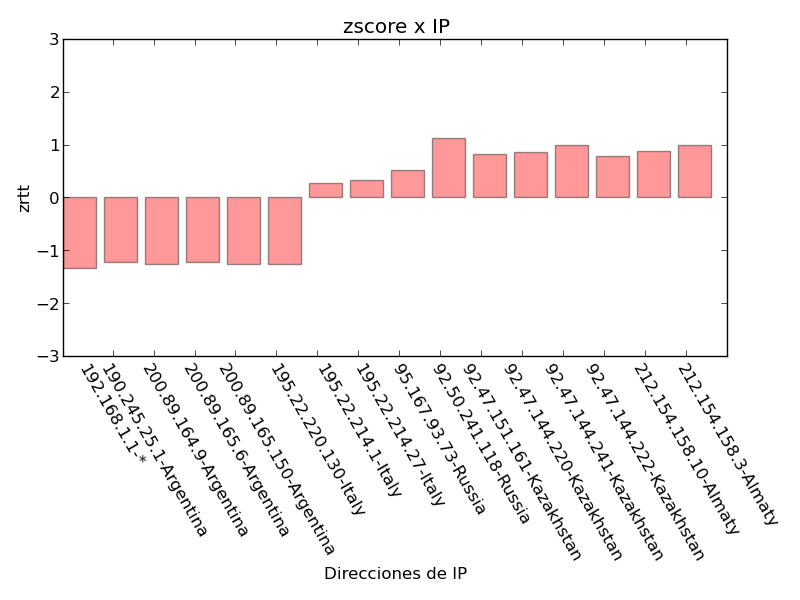
\includegraphics[scale=0.5]{../graficos_informe/aipet_zscore.png}
		  \caption{ZRTT para cada Gateway}
		  \label{fig:contra1}
	\end{center}
\end{figure}

Al igual que para las universidades anteriores puede observarse la gran diferencia del ZRTT antes y luego de pasar el enlace submarino.

\begin{figure}[H]
	\begin{center}
		  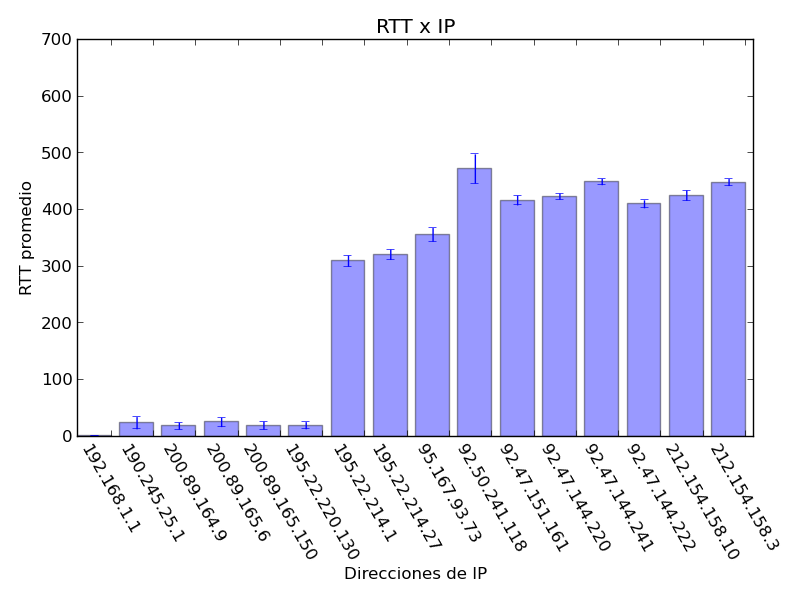
\includegraphics[scale=0.5]{../graficos_informe/aipet_rtt.png}
		  \caption{RTT promedio para cada Gateway con el respectivo desvío estándar}
		  \label{fig:contra1}
	\end{center}
\end{figure}

\begin{figure}[H]
	\begin{center}
		  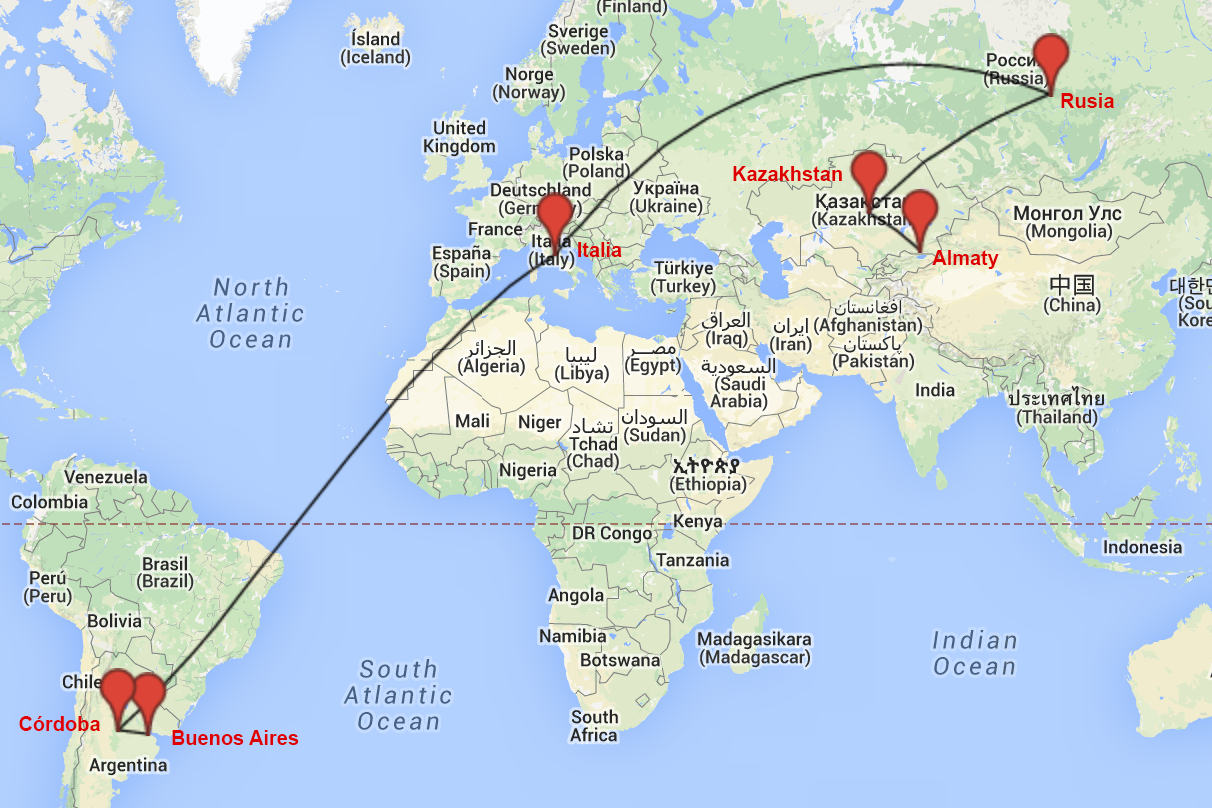
\includegraphics[scale=0.4]{../mapas/mapa_aipet.png}
		  \caption{Mapa de la ruta atravesada para llegar a la universidad de Kazakhstan}
		  \label{fig:contra1}
	\end{center}
\end{figure}

\subsection{Determinación del umbral}

Teniendo en cuenta los resultados obtenidos para cada facultad pudimos observar que el valor de ZRTT calculado para cada Gateway definía bastante bien si se trataba de un enlace submarino o no. En la totalidad de los casos evaluados, un valor de ZRTT positivo nos indicaba la presencia de un enlace submarino por lo cual con determinar $u>0$ nos alcanza para detectarlos.

\subsection{RTT teórico vs RTT experimental}

\subsection{Ping vs RTT's calculados}

Para cada facultad decidimos comparar el valor de RTT obtenido por la $tool$ implementada con lo que retorna el comando $ping$. A continuación los resultados:

Ping a Universidad de Australia:
\begin{verbatim}
PING www.mq.edu.au (137.111.223.158) 56(84) bytes of data.
64 bytes from survivor.mq.edu.au (137.111.223.158): icmp_req=1 ttl=238 time=451 ms
64 bytes from survivor.mq.edu.au (137.111.223.158): icmp_req=2 ttl=238 time=519 ms
64 bytes from survivor.mq.edu.au (137.111.223.158): icmp_req=3 ttl=238 time=492 ms
64 bytes from survivor.mq.edu.au (137.111.223.158): icmp_req=4 ttl=238 time=547 ms
64 bytes from survivor.mq.edu.au (137.111.223.158): icmp_req=5 ttl=238 time=471 ms
64 bytes from survivor.mq.edu.au (137.111.223.158): icmp_req=6 ttl=238 time=533 ms
64 bytes from survivor.mq.edu.au (137.111.223.158): icmp_req=7 ttl=238 time=502 ms
64 bytes from survivor.mq.edu.au (137.111.223.158): icmp_req=8 ttl=238 time=506 ms
64 bytes from survivor.mq.edu.au (137.111.223.158): icmp_req=9 ttl=238 time=464 ms
64 bytes from survivor.mq.edu.au (137.111.223.158): icmp_req=10 ttl=238 time=525 ms
64 bytes from survivor.mq.edu.au (137.111.223.158): icmp_req=11 ttl=238 time=469 ms
64 bytes from survivor.mq.edu.au (137.111.223.158): icmp_req=12 ttl=238 time=524 ms
\end{verbatim}

Ping a Universidad de Kamchatka:

\begin{verbatim}
PING ns.kamgu.ru (85.28.217.202) 56(84) bytes of data.
64 bytes from ns.kamgu.ru (85.28.217.202): icmp_req=1 ttl=48 time=953 ms
64 bytes from ns.kamgu.ru (85.28.217.202): icmp_req=2 ttl=48 time=946 ms
64 bytes from ns.kamgu.ru (85.28.217.202): icmp_req=3 ttl=48 time=962 ms
64 bytes from ns.kamgu.ru (85.28.217.202): icmp_req=4 ttl=48 time=951 ms
64 bytes from ns.kamgu.ru (85.28.217.202): icmp_req=5 ttl=48 time=962 ms
64 bytes from ns.kamgu.ru (85.28.217.202): icmp_req=6 ttl=48 time=946 ms
64 bytes from ns.kamgu.ru (85.28.217.202): icmp_req=7 ttl=48 time=951 ms
64 bytes from ns.kamgu.ru (85.28.217.202): icmp_req=8 ttl=48 time=963 ms
64 bytes from ns.kamgu.ru (85.28.217.202): icmp_req=9 ttl=48 time=965 ms
64 bytes from ns.kamgu.ru (85.28.217.202): icmp_req=10 ttl=48 time=968 ms
64 bytes from ns.kamgu.ru (85.28.217.202): icmp_req=11 ttl=48 time=946 ms
64 bytes from ns.kamgu.ru (85.28.217.202): icmp_req=12 ttl=48 time=974 ms
64 bytes from ns.kamgu.ru (85.28.217.202): icmp_req=13 ttl=48 time=951 ms
\end{verbatim}

Ping a Universidad de Kazajistán:

\begin{verbatim}
PING mail.aipet.kz (212.154.158.3) 56(84) bytes of data.
64 bytes from mail.aipet.kz (212.154.158.3): icmp_req=1 ttl=242 time=371 ms
64 bytes from mail.aipet.kz (212.154.158.3): icmp_req=2 ttl=242 time=349 ms
64 bytes from mail.aipet.kz (212.154.158.3): icmp_req=3 ttl=242 time=360 ms
64 bytes from mail.aipet.kz (212.154.158.3): icmp_req=4 ttl=242 time=363 ms
64 bytes from mail.aipet.kz (212.154.158.3): icmp_req=5 ttl=242 time=356 ms
64 bytes from mail.aipet.kz (212.154.158.3): icmp_req=6 ttl=242 time=368 ms
64 bytes from mail.aipet.kz (212.154.158.3): icmp_req=7 ttl=242 time=351 ms
64 bytes from mail.aipet.kz (212.154.158.3): icmp_req=8 ttl=242 time=356 ms
64 bytes from mail.aipet.kz (212.154.158.3): icmp_req=9 ttl=242 time=348 ms
64 bytes from mail.aipet.kz (212.154.158.3): icmp_req=10 ttl=242 time=354 ms
64 bytes from mail.aipet.kz (212.154.158.3): icmp_req=11 ttl=242 time=355 ms
64 bytes from mail.aipet.kz (212.154.158.3): icmp_req=12 ttl=242 time=354 ms
64 bytes from mail.aipet.kz (212.154.158.3): icmp_req=13 ttl=242 time=354 ms
64 bytes from mail.aipet.kz (212.154.158.3): icmp_req=14 ttl=242 time=369 ms
\end{verbatim}

Los resultados obtenidos por la $tool$ fueron:

\begin{itemize}
	\item Universidad de Autralia: 383.823335171 ms
	\item Universidad de Kamchatka: 963.758111 ms
	\item Universidad de Kazajistán: 448.334944248 ms
\end{itemize}

Como es posible observar, los resultados obtenidos por la $tool$ son bastante parecidos a los de $ping$.